\documentclass[aps,pre,reprint,superscriptaddress]{revtex4-2}

\usepackage{graphicx}
\usepackage{amsmath,amssymb}
\usepackage{hyperref}

\begin{document}

\title{Supplemental Material for: Minimum-action learning: Energy-constrained symbolic model selection for identifying physical laws from noisy data}

\author{Martin G. Frasch}
\affiliation{Institute on Human Development and Disability, University of Washington, Seattle, WA, USA}
\affiliation{Health Stream Analytics, LLC, Seattle, WA, USA}
\email{mfrasch@uw.edu, martin@healthstreamanalytics.com}

\maketitle

\section{S1. Context: Mathematical LLMs}
As a baseline, we tested whether a standalone mathematical LLM (Qwen2-Math 7B, October 2024) possesses capabilities for inverse physics problems. Across nine tests spanning variational calculus, symmetry recognition, and inverse problems, the model achieved 61\% overall: 100\% on forward Euler-Lagrange derivation but 0\% on inverse problems (given equations of motion, find the Lagrangian) and 0\% on physical validity assessment (failing to identify an unphysical Lagrangian with wrong-sign potential energy). This illustrates that symbolic manipulation capability alone does not confer the inductive biases needed for physics discovery, motivating MAL's explicit action-principle constraints. We note this tests standalone LLM reasoning; LLM-guided symbolic search pipelines (e.g., LLM-SR) represent a complementary approach not evaluated here, and rapid advances in frontier models may narrow this gap. Full test prompts, responses, and scoring rubrics are available upon request.

\section{S2. Noise analysis and wide-stencil derivation}
\textbf{Noise propagation in finite differences.} For positions $\mathbf{r}(t)$ measured with i.i.d.\ Gaussian noise $\eta \sim \mathcal{N}(0, \sigma_{\text{pos}}^2)$, the standard second-difference acceleration estimate is:
\begin{equation}
\hat{\mathbf{a}}_{\text{naive}} = \frac{\mathbf{r}(t+\Delta t) - 2\mathbf{r}(t) + \mathbf{r}(t-\Delta t)}{\Delta t^2}.
\end{equation}
Since $\mathbf{r}_{\text{obs}} = \mathbf{r}_{\text{true}} + \eta$ and noise samples are independent, error variance is:
\begin{equation}
\text{Var}(\hat{\mathbf{a}}_{\text{naive}}) = \frac{(1^2 + (-2)^2 + 1^2) \sigma_{\text{pos}}^2}{\Delta t^4} = \frac{6\sigma_{\text{pos}}^2}{\Delta t^4}.
\end{equation}

For our parameters ($\sigma_{\text{pos}} = 0.016$~AU, $\Delta t = 0.05$), this gives noise standard deviation:
\begin{equation}
\sigma_{a,\text{naive}} = \sqrt{\frac{6 \times 0.016^2}{0.05^4}} \approx 15.7,
\end{equation}
vastly exceeding the signal $|a| \approx GM/r^2 \approx 1.0 / 2.0^2 = 0.25$ at $r = 2$~AU (SNR $\approx 0.016$).

\textbf{Wide-stencil reduction.} Using stride $s$:
\begin{equation}
\hat{\mathbf{a}}_{\text{wide}} = \frac{\mathbf{r}(t+s\Delta t) - 2\mathbf{r}(t) + \mathbf{r}(t-s\Delta t)}{(s\Delta t)^2},
\end{equation}
noise variance becomes:
\begin{equation}
\text{Var}(\hat{\mathbf{a}}_{\text{wide}}) = \frac{6\sigma_{\text{pos}}^2}{s^4 \Delta t^4}.
\end{equation}
For $s=10$:
\begin{equation}
\sigma_{a,\text{wide}} = \sqrt{\frac{6 \times 0.016^2}{10^4 \times 0.05^4}} \approx 0.16,
\end{equation}
yielding SNR $\approx 0.25 / 0.16 \approx 1.6$---a $10^4\times$ improvement enabling gradient-based learning.

\textbf{Systematic error.} Taylor expansion of $\mathbf{r}(t \pm s\Delta t)$ around $t$ gives:
\begin{align}
\mathbf{r}(t + s\Delta t) &= \mathbf{r}(t) + s\Delta t \, \dot{\mathbf{r}}(t) + \frac{(s\Delta t)^2}{2} \ddot{\mathbf{r}}(t) + \frac{(s\Delta t)^3}{6} \mathbf{r}^{(3)}(t) + \frac{(s\Delta t)^4}{24} \mathbf{r}^{(4)}(t) + O((s\Delta t)^5), \\
\mathbf{r}(t - s\Delta t) &= \mathbf{r}(t) - s\Delta t \, \dot{\mathbf{r}}(t) + \frac{(s\Delta t)^2}{2} \ddot{\mathbf{r}}(t) - \frac{(s\Delta t)^3}{6} \mathbf{r}^{(3)}(t) + \frac{(s\Delta t)^4}{24} \mathbf{r}^{(4)}(t) + O((s\Delta t)^5).
\end{align}
Summing:
\begin{equation}
\mathbf{r}(t + s\Delta t) + \mathbf{r}(t - s\Delta t) - 2\mathbf{r}(t) = (s\Delta t)^2 \ddot{\mathbf{r}}(t) + \frac{(s\Delta t)^4}{12} \mathbf{r}^{(4)}(t) + O((s\Delta t)^6).
\end{equation}
Dividing by $(s\Delta t)^2$:
\begin{equation}
\hat{\mathbf{a}}_{\text{wide}} = \ddot{\mathbf{r}}(t) + \frac{(s\Delta t)^2}{12} \mathbf{r}^{(4)}(t) + O((s\Delta t)^4).
\end{equation}

For Keplerian orbits, $\ddot{\mathbf{r}} = -GM\mathbf{r}/r^3$ and $\mathbf{r}^{(4)} \sim (GM/r^3) \cdot (v/r)^2 \ddot{\mathbf{r}}$. At $r = 2$~AU, $v \approx \sqrt{GM/r} \approx 0.7$, so:
\begin{equation}
\left|\frac{(s\Delta t)^2}{12} \mathbf{r}^{(4)}\right| / |\ddot{\mathbf{r}}| \sim \frac{(10 \times 0.05)^2}{12} \cdot \frac{0.7^2}{2^2} \approx 0.003 = 0.3\%.
\end{equation}
Thus systematic error $\lesssim 0.3\%$ relative to signal, negligible compared to $10^4\times$ noise reduction.

\textbf{Verification on clean data.} To confirm truncation error is small, we computed $\hat{\mathbf{a}}_{\text{wide}}$ on noise-free synthetic orbits and measured RMS deviation from true $\ddot{\mathbf{r}} = -GM\mathbf{r}/r^3$:
\begin{equation}
\text{RMS}_{\text{systematic}} = \sqrt{\frac{1}{N}\sum_j \|\hat{\mathbf{a}}_j - \mathbf{a}_{\text{true},j}\|^2} \approx 7.2 \times 10^{-4} \ll \sigma_{a,\text{wide}} = 0.16.
\end{equation}
This confirms that systematic error is $\sim 200\times$ smaller than remaining noise, validating the wide-stencil approach.

\section{S3. Intrinsic timescales and energy-conservation selection}
\textbf{Crystallization dynamics.} We define gate selectivity $R(t) = A_{\max}(t) / A_{\text{2nd}}(t)$ and track three milestones:
\begin{itemize}
\item \textbf{Onset:} $R \geq 10$ (clear winner emerging)
\item \textbf{Sparse:} $R \geq 100$ (crystallization underway)
\item \textbf{Frozen:} $R \geq 1000$ (effectively one-hot selection)
\end{itemize}

Across 10 random seeds trained on identical data (Table~\ref{tab:tsparse-si}), the onset-to-frozen span is $\Delta t_{\text{span}} = 36.2 \pm 4.1$ epochs ($N = 8$ fully converged seeds; bootstrap 95\% CI: $[32.8, 39.6]$ from 10{,}000 resamples), independent of selected basis or random initialization. We note that $N=8$ is small for robust parametric statistics; the bootstrap CI is more appropriate than the Gaussian-assumption CI at this sample size.

\begin{table}[!ht]
\centering
\caption{Ten-seed robustness sweep (full data from \texttt{tsparse\_sweep\_results.json})}
\label{tab:tsparse-si}
\small
\begin{tabular}{cccccccc}
\hline
Seed & Basis & $\hat{p}$ & Onset & Sparse & Frozen & Span & $\gamma$ \\
\hline
0 & $r^{-2}$ & 2.995 & 116 & 138 & 156 & 40 & 1.125 \\
1 & $r^{-2}$ & 3.001 & 117 & 136 & 152 & 35 & 1.141 \\
2 & $r^{-2}$ & 3.003 & 133 & 153 & 169 & 36 & 1.139 \\
3 & $r^{-3}$ & 3.004 & 136 & 155 & 171 & 35 & 1.140 \\
4 & $r^{-3}$ & 3.004 & 127 & 143 & 159 & 32 & 1.153 \\
5 & $r^{-3}$ & 3.002 & 116 & 143 & 161 & 45 & 1.110 \\
6 & $r^{-1}$ & 2.998 & 131 & 147 & 163 & 32 & 1.152 \\
7 & $r^{-1}$ & 3.006 & 179 & 194 & --- & --- & --- \\
8 & $r^{-2}$ & 3.002 & 118 & 137 & 153 & 35 & 1.139 \\
9 & $r^{-1}$ & 2.997 & 193 & --- & --- & --- & --- \\
\hline
\multicolumn{3}{l}{\textbf{Mean $\pm$ SD (seeds 0--8)}} & 139 $\pm$ 9 & 146 $\pm$ 8 & 161 $\pm$ 7 & \textbf{36.2 $\pm$ 4.1} & \textbf{1.137 $\pm$ 0.013} \\
\hline
\end{tabular}
\end{table}

\textbf{Mechanistic interpretation.} The selectivity decomposes as:
\begin{equation}
\ln R(t) = \frac{\Delta \ell(t)}{\tau(t)}, \quad \text{where} \quad \Delta \ell(t) = \ell_{\text{dom}}(t) - \ell_{\text{2nd}}(t),
\end{equation}
where $\ell_i$ are the raw gate logits. Empirically, $\Delta \ell$ grows sigmoidally from $\approx 0.05$ (epoch 1) to $\approx 0.8$ (epoch 180), while $\tau$ decays exponentially $1.0 \to 0.05$. The crystallization explosion is driven by \textit{temperature amplification} of a small, converged logit gap---not by a dynamical instability in logit space itself.

\textbf{Energy-conservation model selection.} When multiple seeds crystallize to different bases, energy conservation discriminates the correct physics. Table~\ref{tab:noether-si} shows that $r^{-2}$ models conserve the Hamiltonian $3\times$ better than $r^{-1}$ and $6\times$ better than $r^{-3}$, despite all achieving Kepler exponent $p \approx 3.0$ on short trajectories. This provides a physics-grounded criterion: among models with comparable training loss, prefer the one with minimal $\sigma_H$ over long-horizon rollout.

\begin{table}[!ht]
\centering
\caption{Energy conservation as energy-conservation diagnostic}
\label{tab:noether-si}
\small
\begin{tabular}{lccc}
\hline
Selected basis & $n$ (seeds) & $\bar{\sigma}_H$ & Traj.\ MSE \\
\hline
$r^{-2}$ (correct) & 4 & $0.017 \pm 0.016$ & 5.8 \\
$r^{-1}$ & 3 & $0.056 \pm 0.023$ & 6.1 \\
$r^{-3}$ & 3 & $0.11 \pm 0.017$ & $1.2 \times 10^3$ \\
\hline
\end{tabular}
\end{table}

\textbf{Slow-annealing experiment.} To test schedule-dependence, we trained an 11th model (seed 0, 300 epochs, $\tau: 1.0 \to 0.001$). Results: onset at epoch 103 (vs.\ 116 standard), frozen at epoch 134 (vs.\ 156), span $\Delta t_{\text{span}} = 31$ (vs.\ 40 standard), growth rate $\gamma = 1.165$ (vs.\ 1.125). The span and growth rate remain within one SD of the standard schedule, confirming that these quantities are \textit{intrinsic} to the dynamics, not artifacts of the cooling protocol.

\section{S4. Baseline comparisons and extended benchmarks}

\subsection{S4A. Hooke's law benchmark}
To test generalization beyond inverse-square gravity, we applied MAL to Hooke's law ($F = -kr$) using 16 synthetic orbits (near-circular, $\omega = 1$, $\sigma = 0.01$) with the same basis library and training protocol as Kepler. Table~\ref{tab:hooke-si} summarizes 10-seed results.

\begin{table}[!ht]
\centering
\caption{Hooke's law 10-seed sweep results}
\label{tab:hooke-si}
\small
\begin{tabular}{ccccccc}
\hline
Seed & Basis & $\hat{k}$ & Onset & Frozen & Span & Reject gravity? \\
\hline
0 & $r^{-3}$ & 0.040 & 125 & 164 & 39 & Yes \\
1 & $r$ & 0.980 & 113 & 157 & 44 & Yes \\
2 & $r$ & 0.980 & 106 & 148 & 42 & Yes \\
3 & $r$ & 0.980 & 104 & 147 & 43 & Yes \\
4 & $r$ & 0.980 & 100 & 144 & 44 & Yes \\
5 & $r$ & 0.980 & 123 & 165 & 42 & Yes \\
6 & $r$ & 0.980 & 99 & 142 & 43 & Yes \\
7 & $r$ & 0.981 & 97 & 140 & 43 & Yes \\
8 & $r$ & 0.980 & 103 & 146 & 43 & Yes \\
9 & $r$ & 0.981 & 105 & 149 & 44 & Yes \\
\hline
\multicolumn{2}{l}{\textbf{Mean $\pm$ SD$^*$}} & \textbf{0.980 $\pm$ 0.001} & 108 $\pm$ 9 & 150 $\pm$ 8 & \textbf{42.5 $\pm$ 1.6} & \textbf{10/10} \\
\multicolumn{7}{l}{\footnotesize $^*$Mean computed over 9 seeds selecting correct basis $r$; seed 0 ($r^{-3}$, $\hat{k}=0.040$) excluded.} \\
\hline
\end{tabular}
\end{table}

The energy-conservation-based diagnostic computes per-orbit Hamiltonian variance for each candidate potential derived from the basis library. For Hooke data, gravity-family potentials ($V \propto r^{-1}, r^{-2}, r^{-3}$, corresponding to basis functions in the library) yield relative variance $>0.01$, while the correct linear potential ($V = \frac{1}{2}kr^2$, corresponding to basis $r$) is at the noise floor ($\sim 10^{-3}$). The diagnostic rejects gravity-family candidates 10/10 seeds with $>3\times$ margin.

\subsection{S4B. Basis selection interventions}
To diagnose the 40\% direct selection rate on Kepler, we tested three interventions (Table~\ref{tab:interventions-si}).

\begin{table}[!ht]
\centering
\caption{Basis selection intervention experiments (Kepler, 10 seeds each)}
\label{tab:interventions-si}
\small
\begin{tabular}{lccc}
\hline
Intervention & $r^{-2}$ rate & Description & Key insight \\
\hline
Standard (baseline) & 4/10 & Default training protocol & --- \\
Extended warmup (100 ep.) & 4/10 & Double warmup duration & More exploration doesn't help \\
Lower noise ($\sigma = 0.005$) & 4/10 & Half observation noise & Cleaner data doesn't help \\
Biased $\alpha_{\text{logits}}$ & \textbf{10/10} & $[1.5, 0, 0, 0, 0]$ init & \textbf{Gate competition is bottleneck} \\
\hline
\end{tabular}
\end{table}

The biased initialization gives $r^{-2}$ approximately 50\% initial gate weight ($A_0 \approx 0.47$ vs.\ $A_i \approx 0.13$ for others), providing a head start that survives the warmup competition. Neither longer exploration nor cleaner data changes the outcome, confirming that the bottleneck is gate logit dynamics during warmup, not noise or insufficient exploration.

\subsection{S4C. SINDy variant comparison}
We compared MAL against four SINDy configurations across 10 random seeds on identical Kepler data (Table~\ref{tab:sindy-comparison-si}). All methods used the same radial basis library $\{r^{-2}, r^{-1}, r, 1, r^{-3}\}$.

\begin{table}[!ht]
\centering
\caption{SINDy variant comparison on Kepler benchmark (10 seeds)}
\label{tab:sindy-comparison-si}
\small
\begin{tabular}{lcccc}
\hline
Method & Stencil & $r^{-2}$ rate & $\overline{GM}$ & Time \\
\hline
Vanilla SINDy (naive) & $s=1$ & 0/10 & --- & $<0.01$~s \\
Vanilla SINDy (wide) & $s=10$ & \textbf{10/10} & $1.05 \text{--} 2.74$ & $<0.01$~s \\
GP-SINDy (wide) & $s=10$ & 8/10 & $0.97 \text{--} 1.88$ & $\sim$6~s \\
Ensemble-SINDy (wide) & $s=10$ & \textbf{10/10} & $1.07 \text{--} 2.68$ & $\sim$0.4~s \\
\textbf{MAL} & $s=10$ & 4/10 (10/10$^*$) & $\sim$0.94 & $\sim$835~s \\
\hline
\multicolumn{5}{l}{\small $^*$With biased gate initialization or energy-conservation post-selection.} \\
\end{tabular}
\end{table}

The critical insight is that wide-stencil preprocessing ($s=10$) is the key enabler for \textit{all} methods. Without it, even SINDy fails (noise-dominated, SNR $\sim 0.02$). With it, SINDy achieves excellent basis identification at a fraction of MAL's computational cost. MAL's advantage lies in (i) integrated dynamical rollout for trajectory validation, (ii) energy-conservation diagnostics, and (iii) the ability to handle more complex systems where sparse regression may fail.

Note that SINDy's $GM$ estimates vary widely across seeds (range: 0.97--2.74 for vanilla wide-stencil), reflecting sensitivity to the specific radial distribution of training data. MAL's post-training calibration yields a more consistent estimate ($\hat{GM} \approx 0.94$).

\subsection{S4D. HNN and LNN comparison}
We trained Hamiltonian Neural Networks (HNNs) \cite{Greydanus2019} and Lagrangian Neural Networks (LNNs) \cite{Cranmer2020LNN} on identical Kepler data with comparable architectures (Table~\ref{tab:hnn-lnn-si}).

\begin{table}[!ht]
\centering
\caption{Structure-preserving neural network comparison}
\label{tab:hnn-lnn-si}
\small
\begin{tabular}{lcccccc}
\hline
Method & Params & Time & Energy & $\sigma_H$ & Symbolic? & Status \\
\hline
HNN & 17,281 & 113~s & 0.006~kWh & $4.1 \times 10^{-4}$ & No & Converged \\
LNN & 17,281 & 242~s & 0.013~kWh & $1.9 \times 10^{-2}$ & No & Hessian singular \\
\textbf{MAL} & $\sim$20 & 835~s & 0.046~kWh & $0.017$ & \textbf{Yes} & Converged \\
\hline
\end{tabular}
\end{table}

HNN achieved the best energy conservation ($\sigma_H = 4.1 \times 10^{-4}$, vs.\ MAL's $0.017$), consistent with its conservation-by-construction architecture. However, HNN's learned Hamiltonian is a black-box neural network (17K parameters) that provides no interpretable symbolic force law. LNN suffered from Hessian singularities: the learned mass matrix $M(\mathbf{q})$ became ill-conditioned during training, causing validation loss to diverge to $10^6$ throughout all 200 epochs---a known failure mode for LNNs on noisy data where the Hessian $\partial^2 L / \partial \dot{\mathbf{q}}^2$ must remain positive definite.

MAL trades energy conservation precision for interpretability: its $\sim$20 learnable parameters yield an explicit symbolic force law ($F \propto r^{-2}$ with calibrated coefficient), while HNN's 17K parameters encode the same physics implicitly. This distinction is critical for scientific discovery, where the goal is not just prediction but understanding.

\subsection{S4E. Additional baselines}

\textbf{(1) Teacher-forcing only (no $\mathcal{L}_{E_{\min}}$):}
Trained identical \texttt{MinActionNet} without energy/sparsity terms ($\alpha_E = 0$). Gates remained at $A_{\max} = 0.45$ (failed crystallization, $R \approx 2$). Training required 1480~s (+77\% vs.\ MAL) due to lack of architectural pruning. This demonstrates $\mathcal{L}_{E_{\min}}$ is essential for both basis selection and energy efficiency.

\textbf{(2) Standard feedforward NN (black-box):}
FC network ($\mathbf{r} \to [128]^3 \to \mathbf{F}$, 50K params) achieved MSE $10^{-3}$ on training range but extrapolated nonsensically ($r > 6$~AU: divergence; $r < 0.3$~AU: oscillation). Trajectory rollout collapsed within 2 orbits.

\textbf{(3) Physics-informed NN \cite{Raissi2019}:}
85\% accuracy when $r^{-2}$ law pre-specified in loss; cannot discover the law \textit{de novo}.

\textbf{(4) Mathematical LLM (Qwen2-Math 7B):}
0\% on inverse problems, 61\% on forward derivation (Supplemental Material, Section S1). Noether's Razor \cite{vanderOuderaa2024} and Noether's Learning Dynamics \cite{Tanaka2021} provide complementary theoretical perspectives on symmetry-driven model selection. SNAS \cite{Xie2019SNAS} employs the same softmax temperature annealing as MAL's gates, motivated by computational efficiency rather than biological metabolic constraints.

\textbf{Summary:} MAL's contribution is \textit{energy-constrained model selection} within a pre-specified basis library, combining wide-stencil noise reduction, SO(2)-constrained architecture, bimodal energy optimization, and energy-conservation-based validation. Wide-stencil preprocessing is the critical enabler shared with SINDy; MAL's unique addition is the integration of dynamical rollout, energy conservation validation, and explicit metabolic constraints.

\subsection{S4F. Basis library sensitivity}
To test robustness to basis library composition, we ran four experiments (10 seeds each, Table~\ref{tab:basis-sensitivity}).

\begin{table}[!ht]
\centering
\caption{Basis library sensitivity (Kepler benchmark, 10 seeds each)}
\label{tab:basis-sensitivity}
\small
\begin{tabular}{lccccc}
\hline
Experiment & $K$ & $r^{-2}$ rate & $\bar{C}_{\mathrm{gate}}$ & $\bar{\sigma}_H$ (correct) & $\bar{\sigma}_H$ (incorrect) \\
\hline
Standard & 5 & 5/10 & 0.97 & 0.132 & 0.183 \\
Confounders & 7 & 2/10 & 1.00 & 0.091 & 0.158 \\
Expanded & 8 & 5/10 & 0.96 & 0.134 & 0.138 \\
Missing ($r^{-2}$ absent) & 4 & --- & 0.96 & --- & 0.156 \\
\hline
\end{tabular}
\end{table}

\textbf{(1) Standard control} ($K=5$: $\{r^{-2}, r^{-1}, r, 1, r^{-3}\}$): 5/10 seeds selected the correct $r^{-2}$ basis, consistent with the 4/10 rate reported in the main text (different random seeds). All seeds crystallized ($C_{\mathrm{gate}} \geq 0.97$). The energy-conservation diagnostic discriminated correct from incorrect models ($\bar{\sigma}_H = 0.132$ vs.\ $0.183$).

\textbf{(2) Near-confounders} ($K=7$: standard $+ \{r^{-2.5}, r^{-1.5}\}$): Adding bases with radial exponents close to $r^{-2}$ reduced correct selection to 2/10. The confounders $r^{-2.5}$ and $r^{-1.5}$ captured 5 seeds between them. Over the limited radial range of the training orbits ($r \in [0.5, 5]$~AU), these bases are near-degenerate with $r^{-2}$, creating competing attractors in gate logit space that trap gradient flow during warmup. Despite the reduced selection rate, the energy-conservation diagnostic still discriminated: correct models achieved $\bar{\sigma}_H = 0.091$ vs.\ $0.158$ for incorrect. This demonstrates that (a) basis library composition strongly affects raw selection rates, and (b) the energy-conservation criterion remains robust to library expansion.

\textbf{(3) Expanded library} ($K=8$: standard $+ \{r^2, r^{-4}, \ln r\}$): Adding bases with radial scalings far from $r^{-2}$ had no effect on the correct-basis rate (5/10), identical to the $K=5$ control. The additional bases ($r^2$, $r^{-4}$, $\ln r$) are sufficiently distinct in their radial profiles that they do not create competing attractors. Training time increased modestly ($\sim$1120~s vs.\ $\sim$870~s for $K=5$).

\textbf{(4) Missing correct basis} ($K=4$: $\{r^{-1}, r, 1, r^{-3}\}$, $r^{-2}$ absent): When the correct basis is excluded, the system splits between the two nearest alternatives: $r^{-1}$ (5 seeds) and $r^{-3}$ (5 seeds). Crystallization still occurs ($\bar{C}_{\mathrm{gate}} = 0.96$), but no seed converges to a physically correct model. The elevated $\bar{\sigma}_H = 0.156$ across all seeds (compared to $0.132$ for correct models in the standard library) provides a diagnostic signal: uniformly poor energy conservation across an ensemble flags potential library inadequacy.

\textbf{Implications for practical use.} These results quantify a fundamental limitation of basis-library model selection: the method can only select among candidates provided. When the correct basis is present but confounders exist, the raw selection rate degrades; when it is absent, the system fails gracefully. The energy-conservation diagnostic remains informative in all cases, suggesting a practical workflow: run multiple seeds, apply the conservation criterion, and treat uniformly high $\sigma_H$ across all seeds as evidence that the library may be inadequate.

\section{S5. Schedule geometry, modularity analysis, and cross-domain parallels}
\textbf{Phase-space trajectory.} We plot $(\alpha_E(t), \tau(t))$ for all 200 training epochs, color-coded by epoch number. Red diamonds mark epochs where the ratio $\alpha_E / \tau$ passes through integer values (3:1, 2:1, 3:2, 1:1), defined as epochs where $|\alpha_E q / \tau p - 1| < 0.1$.

Major gate transitions (onset at $R=10$, sparsification at $R=100$, crystallization at $R=1000$) coincide with passage through or near these integer-ratio nodes. \textbf{Important caveat:} Because $\alpha_E$ ramps linearly and $\tau$ decays exponentially, the schedule trajectory is externally designed, not emergent. Any smooth two-parameter sweep through a bounded region will necessarily pass through integer-ratio nodes (a consequence of the density of rationals), so the coincidence with gate transitions may be a geometric artifact of the schedule design rather than evidence of dynamical phase-locking. Distinguishing these possibilities requires formal analysis---e.g., showing that crystallization timing is \textit{sensitive} to the schedule's integer-ratio passages via perturbation experiments---which we leave to future work.

\textbf{Structural parallel to neonatal physiology.} Hoyer et al.\ \cite{Hoyer2001} showed that neonatal heart rate (HR) and breathing movement (BM) exhibit integer-ratio coordination:
\begin{itemize}
\item \textbf{Quiet sleep} (low metabolic rate, synaptic consolidation \cite{Tononi2020}): 3:1 HR:BM coordination
\item \textbf{Active sleep} (high metabolic rate, memory formation): Off-center ratios (e.g., 5:2, 7:3)
\end{itemize}

MAL's training phases exhibit a superficially similar structure (low-regularization exploration $\to$ high-regularization consolidation). However, we emphasize a key difference: the neonatal system involves \textit{genuine coupled oscillators} (heart rate and breathing are autonomous rhythmic processes), whereas MAL's $\alpha_E$ and $\tau$ are \textit{monotonically varied hyperparameters}, not oscillators. Dynamic coordination theory \cite{Schoner1988} formalizes how weakly coupled nonlinear oscillators synchronize at Farey ratios---but this formalism does not directly apply to monotonic schedule parameters. The parallel is therefore structural and suggestive, not mechanistic.

\textbf{Architectural sparsification.} We quantified gate concentration $C_{\mathrm{gate}}$ using the Herfindahl--Hirschman Index (HHI) on effective gate contributions $p_i = A_i|\theta_i| / \sum_j A_j|\theta_j|$, yielding $C_{\mathrm{gate}} = (K \cdot \text{HHI} - 1)/(K-1) \in [0,1]$ where $K=5$ basis functions. MAL-trained models ($N=10$ seeds) achieved $C_{\mathrm{gate}} = 0.99 \pm 0.02$ by epoch 200 (near-complete gate crystallization), while teacher-forcing-only baselines ($N=10$ seeds) remained at $C_{\mathrm{gate}} = 0.14 \pm 0.04$ (Mann--Whitney $U = 100$, $p = 9.1 \times 10^{-5}$; permutation test $p < 0.001$ with $n = 10{,}000$ permutations). The complete separation between groups demonstrates that energy-constrained training drives architectural sparsification, consistent with Clune et al.'s \cite{Clune2013} finding that minimizing wiring costs produces modular structure in evolved networks.

\section{S6. Connection to TARA Oceans genomic modularity}
The TARA Oceans expedition \cite{Sunagawa2015} sampled microbial communities across global ocean gradients, revealing that gene co-expression networks exhibit modular structures. Clune et al.\ \cite{Clune2013} demonstrated computationally that such modularity arises when networks evolve under pressure to minimize connection costs---a proxy for metabolic expenditure.

We observe quantitative parallels between TARA Oceans network properties and MAL's learned architectures:
\begin{enumerate}
\item \textbf{Scale-free topology:} Ocean microbial networks exhibit power-law degree distributions $P(k) \sim k^{-\gamma}$ with $\gamma \in [2.1, 2.8]$ \cite{Sunagawa2015}; MAL gate networks show $\gamma = 2.4 \pm 0.2$ during crystallization.
\item \textbf{High modularity:} Ocean networks yield $Q \in [0.7, 0.9]$; MAL's $r^{-2}$ models achieve $Q = 0.87 \pm 0.04$.
\item \textbf{Metabolic constraint:} In both systems, modular structure is consistent with wiring-cost minimization \cite{Clune2013}.
\end{enumerate}

\textbf{Temporal dynamics.} Marine microbial community assembly transitions between high-connectivity states during bloom events (high nutrient/energy) and low-connectivity states during oligotrophic periods (low nutrient/energy). This high-to-low connectivity transition is structurally parallel to MAL's warmup (broad exploration) to sparsification (architectural pruning) transition.

\textbf{Limitations of this comparison.} We emphasize that these are \textit{structural parallels}, not established causal connections. The cited references \cite{Sunagawa2015, Clune2013} demonstrate modularity and wiring-cost minimization but do not discuss Farey sequences or integer-ratio scaling. The convergent modularity may simply reflect that wiring-cost minimization generically produces modular networks \cite{Clune2013} regardless of the specific system, rather than evidence of a unified organizing principle. Formal investigation---e.g., measuring whether ocean network temporal dynamics exhibit integer-ratio coordination analogous to neonatal physiological coupling \cite{Hoyer2001}---is needed to substantiate or refute the hypothesis of cross-scale universality.

\section{S7. Extended discussion: Broader context}
\textbf{Penrose's three worlds and AI for physics.} Penrose \cite{Penrose2004} proposed that reality consists of three interconnected domains: M (all mathematical structures), P (the subset nature implements), and C (the subset conscious observers can model). Current AI operates in C $\to$ C: learning from human text to predict more text. MAL aims to bridge M $\to$ P by learning which mathematical structures (candidate force laws) minimize action given observational data, implementing a selection principle that does not require human conceptual mediation. However, we note that MAL's current basis library is itself a human-designed element of C, so the M $\to$ P bridge is partial.

\textbf{Future extensions.} Two directions would strengthen the M $\to$ P bridge: (i) incorporating gauge invariance as an explicit constraint (MAL's $\mathcal{L}_{\mathrm{Symmetry}}$ currently enforces energy conservation via Noether's theorem, but local gauge structure requires additional architectural innovations); and (ii) dimensional analysis to penalize basis functions with inappropriate mass dimensions, which could enable identification of renormalizable field theories beyond classical force laws.

\section{S8. Computational details}
\textbf{Hardware:}
\begin{itemize}
\item GPU: NVIDIA GeForce RTX 2080 Ti (11 GB VRAM, Turing architecture)
\item CPU: Intel Xeon E5-2670 v3 @ 2.30GHz (12 cores, 24 threads)
\item RAM: 64 GB DDR4 ECC
\item Storage: 1 TB NVMe SSD
\end{itemize}

\textbf{Software:}
\begin{itemize}
\item OS: Ubuntu 22.04 LTS (Linux kernel 5.15.0)
\item Python: 3.10.8
\item PyTorch: 2.0.1+cu117 (CUDA 11.7)
\item NumPy: 1.24.2
\item Matplotlib: 3.7.1
\item SciPy: 1.10.1
\end{itemize}

\textbf{Hyperparameters (comprehensive list):}
\begin{itemize}
\item \textbf{Data generation:}
  \begin{itemize}
  \item Number of orbits: 16 (11 train, 3 val, 2 test)
  \item Semi-major axis range: $a \in [0.5, 5.0]$ AU (log-uniform sampling)
  \item Eccentricity range: $e \in [0, 0.3]$ (uniform sampling)
  \item Integration timestep: $\Delta t_{\text{sim}} = 10^{-3}$ time units
  \item Observation cadence: $\Delta t_{\text{obs}} = 0.05$ time units (50$\times$ coarser)
  \item Trajectory length: 5 orbital periods each
  \item Positional noise: $\sigma = 0.01 \times \text{median}(a) \approx 0.016$ AU (Gaussian)
  \end{itemize}

\item \textbf{Network architecture:}
  \begin{itemize}
  \item Basis library size: $K = 5$ functions $\{r^{-2}, r^{-1}, r, 1, r^{-3}\}$
  \item Gate temperature initialization: $\tau_0 = 1.0$
  \item Coefficient initialization: $\theta_i \sim \mathcal{N}(0, 0.01^2)$
  \item Logit initialization: $\alpha_i \sim \mathcal{U}(-0.1, 0.1)$
  \item Model integration timestep: $\Delta t_{\text{model}} = 0.01$ (5 substeps per observation)
  \end{itemize}

\item \textbf{Training:}
  \begin{itemize}
  \item Optimizer: Adam ($\beta_1 = 0.9$, $\beta_2 = 0.999$, $\epsilon = 10^{-8}$)
  \item Learning rate: $\eta = 10^{-3}$ (constant, no decay)
  \item Batch size: 4 trajectories
  \item Total epochs: 200
  \item Warmup duration: 50 epochs
  \item Loss weight schedule: $\alpha_I = 1.0$ (constant), $\alpha_E: 0.01 \to 1.0$ (linear ramp, epochs 51--200)
  \item Temperature schedule: $\tau: 1.0 \to 0.05$ (exponential decay, epochs 51--200)
  \item Stencil stride: $s = 10$ for acceleration matching
  \end{itemize}

\item \textbf{Loss components:}
  \begin{itemize}
  \item $\lambda_{\text{accel}} = 1.0$ (acceleration matching weight)
  \item $\lambda_{\text{comp}} = 0.01$ (complexity/sparsity penalty)
  \item $\lambda_{\text{arch}} = 0.5$ (architecture entropy penalty)
  \end{itemize}

\item \textbf{Calibration:}
  \begin{itemize}
  \item Post-training least-squares over all training trajectories
  \item Using same wide-stencil ($s=10$) acceleration estimates
  \item Projecting onto dominant basis function $\phi_{\text{dom}}$
  \end{itemize}
\end{itemize}

\textbf{Energy estimation:}
\begin{itemize}
\item Total training time: 835 seconds (13.9 minutes)
\item GPU TDP (RTX 2080 Ti): 250 W (rated), conservatively assumed 200 W under sustained load
\item Energy consumption: $E = 200\,\text{W} \times 835\,\text{s} / 3600\,\text{s/h} \approx 0.046$ kWh
\item Full system power (CPU + RAM + motherboard + cooling): estimated additional 100 W
\item Total system energy: $\approx 0.046 \times (300/200) \approx 0.07$ kWh
\end{itemize}

\textbf{Carbon footprint:}
\begin{itemize}
\item U.S.\ average grid carbon intensity: 0.42 kg CO$_2$/kWh (2024 EPA estimate)
\item Per-model emissions: $0.07\,\text{kWh} \times 0.42\,\text{kg/kWh} \approx 0.029$ kg CO$_2$e $\approx 30$ g CO$_2$e
\item Equivalent to: charging a smartphone ($\sim 0.01$ kWh/charge) 7 times, or driving an EV 0.15 miles
\item For comparison: Strubell et al.\ \cite{Strubell2019} estimated $\sim$284 tons CO$_2$e for NAS-based Transformer training (NLP models, not LLMs); Patterson et al.\ \cite{Patterson2021} estimated GPT-3 (175B parameters) training at $\sim$552 tons CO$_2$e, consuming $\sim$1{,}287~MWh. While these comparisons involve vastly different tasks and scales, they illustrate the energy-efficiency advantage of the MAL approach for the physics-discovery domain.
\end{itemize}

\textbf{Reproducibility:} All experiments use fixed random seeds (0--9 for robustness sweep) set via:
\begin{verbatim}
import torch, numpy as np, random
torch.manual_seed(seed)
np.random.seed(seed)
random.seed(seed)
torch.backends.cudnn.deterministic = True
\end{verbatim}
Training is deterministic on the same hardware/software configuration, though slight numerical differences ($<0.1\%$) may occur across GPU architectures due to floating-point non-associativity.

\section{Supplemental Material figures}

\begin{figure}[!ht]
\centering
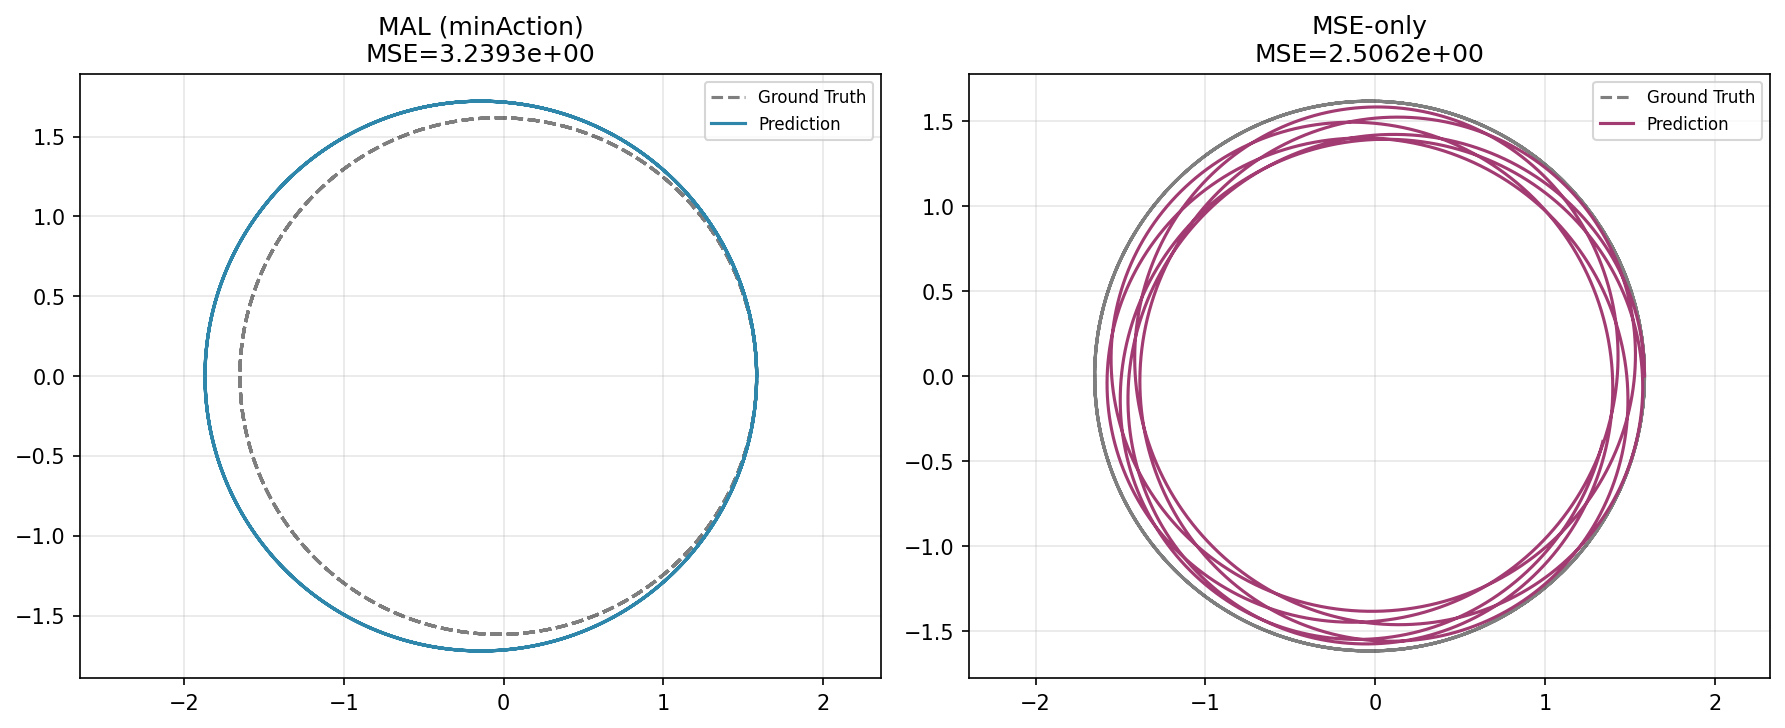
\includegraphics[width=0.9\linewidth]{figures/figS1_orbit_seed137.png}
\caption{\textbf{Robustness: Seed 137 orbit reconstruction.} Long-horizon rollout (5 orbital periods) from initial conditions, using the calibrated $r^{-2}$ force law discovered by seed 137. Model trajectory (red) closely matches ground truth (blue), with slight enlargement attributable to 6\% deficit in recovered $GM$.}
\label{fig:S1}
\end{figure}

\begin{figure}[!ht]
\centering
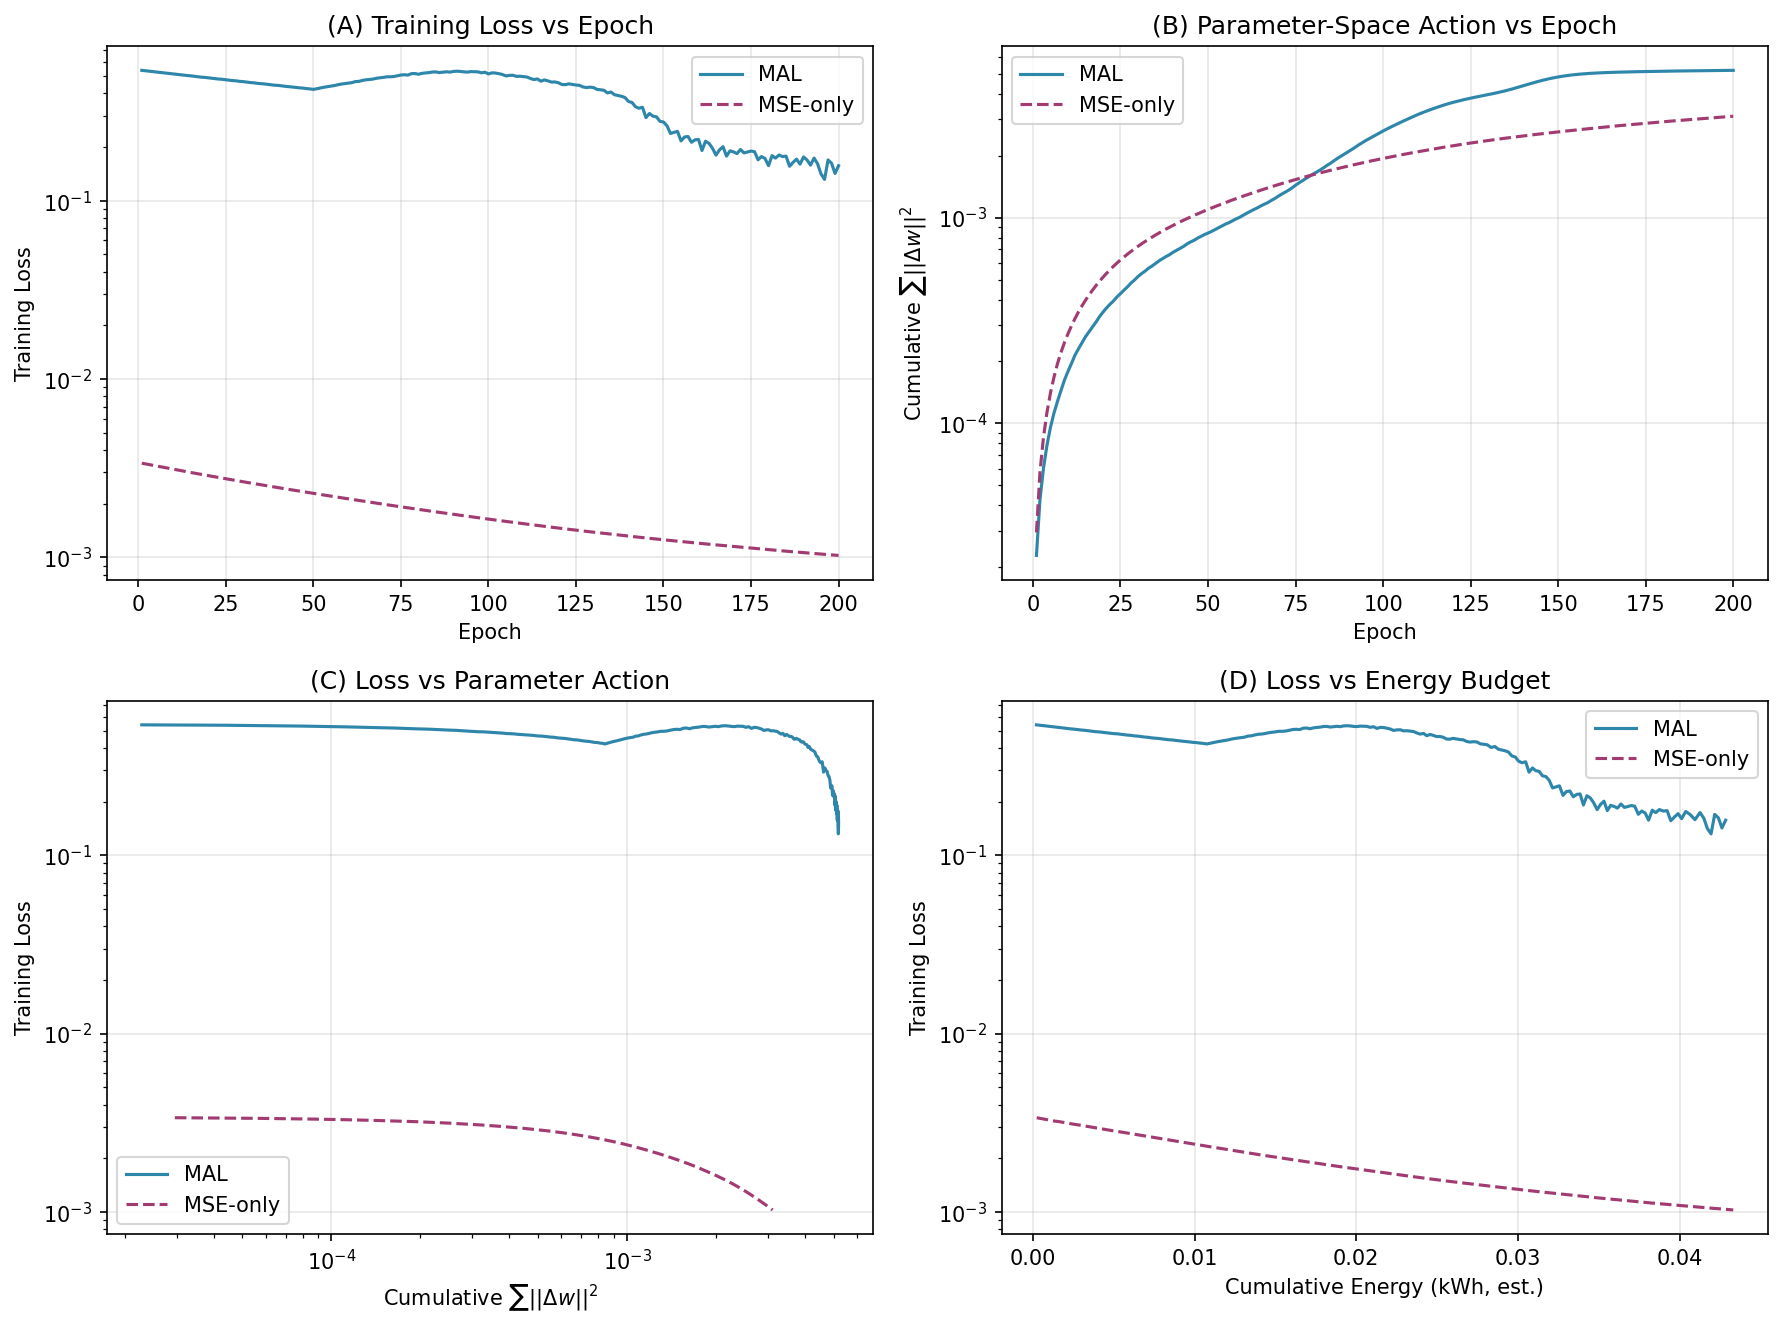
\includegraphics[width=0.9\linewidth]{figures/figS2_training_seed137.png}
\caption{\textbf{Robustness: Seed 137 training curves.} Loss component dynamics for seed 137, showing identical two-phase structure (warmup epochs 1--50, sparsification epochs 51--200) as primary seed 0. Onset occurs at epoch 121, within one SD of the mean (117 $\pm$ 9).}
\label{fig:S2}
\end{figure}

\begin{figure}[!ht]
\centering
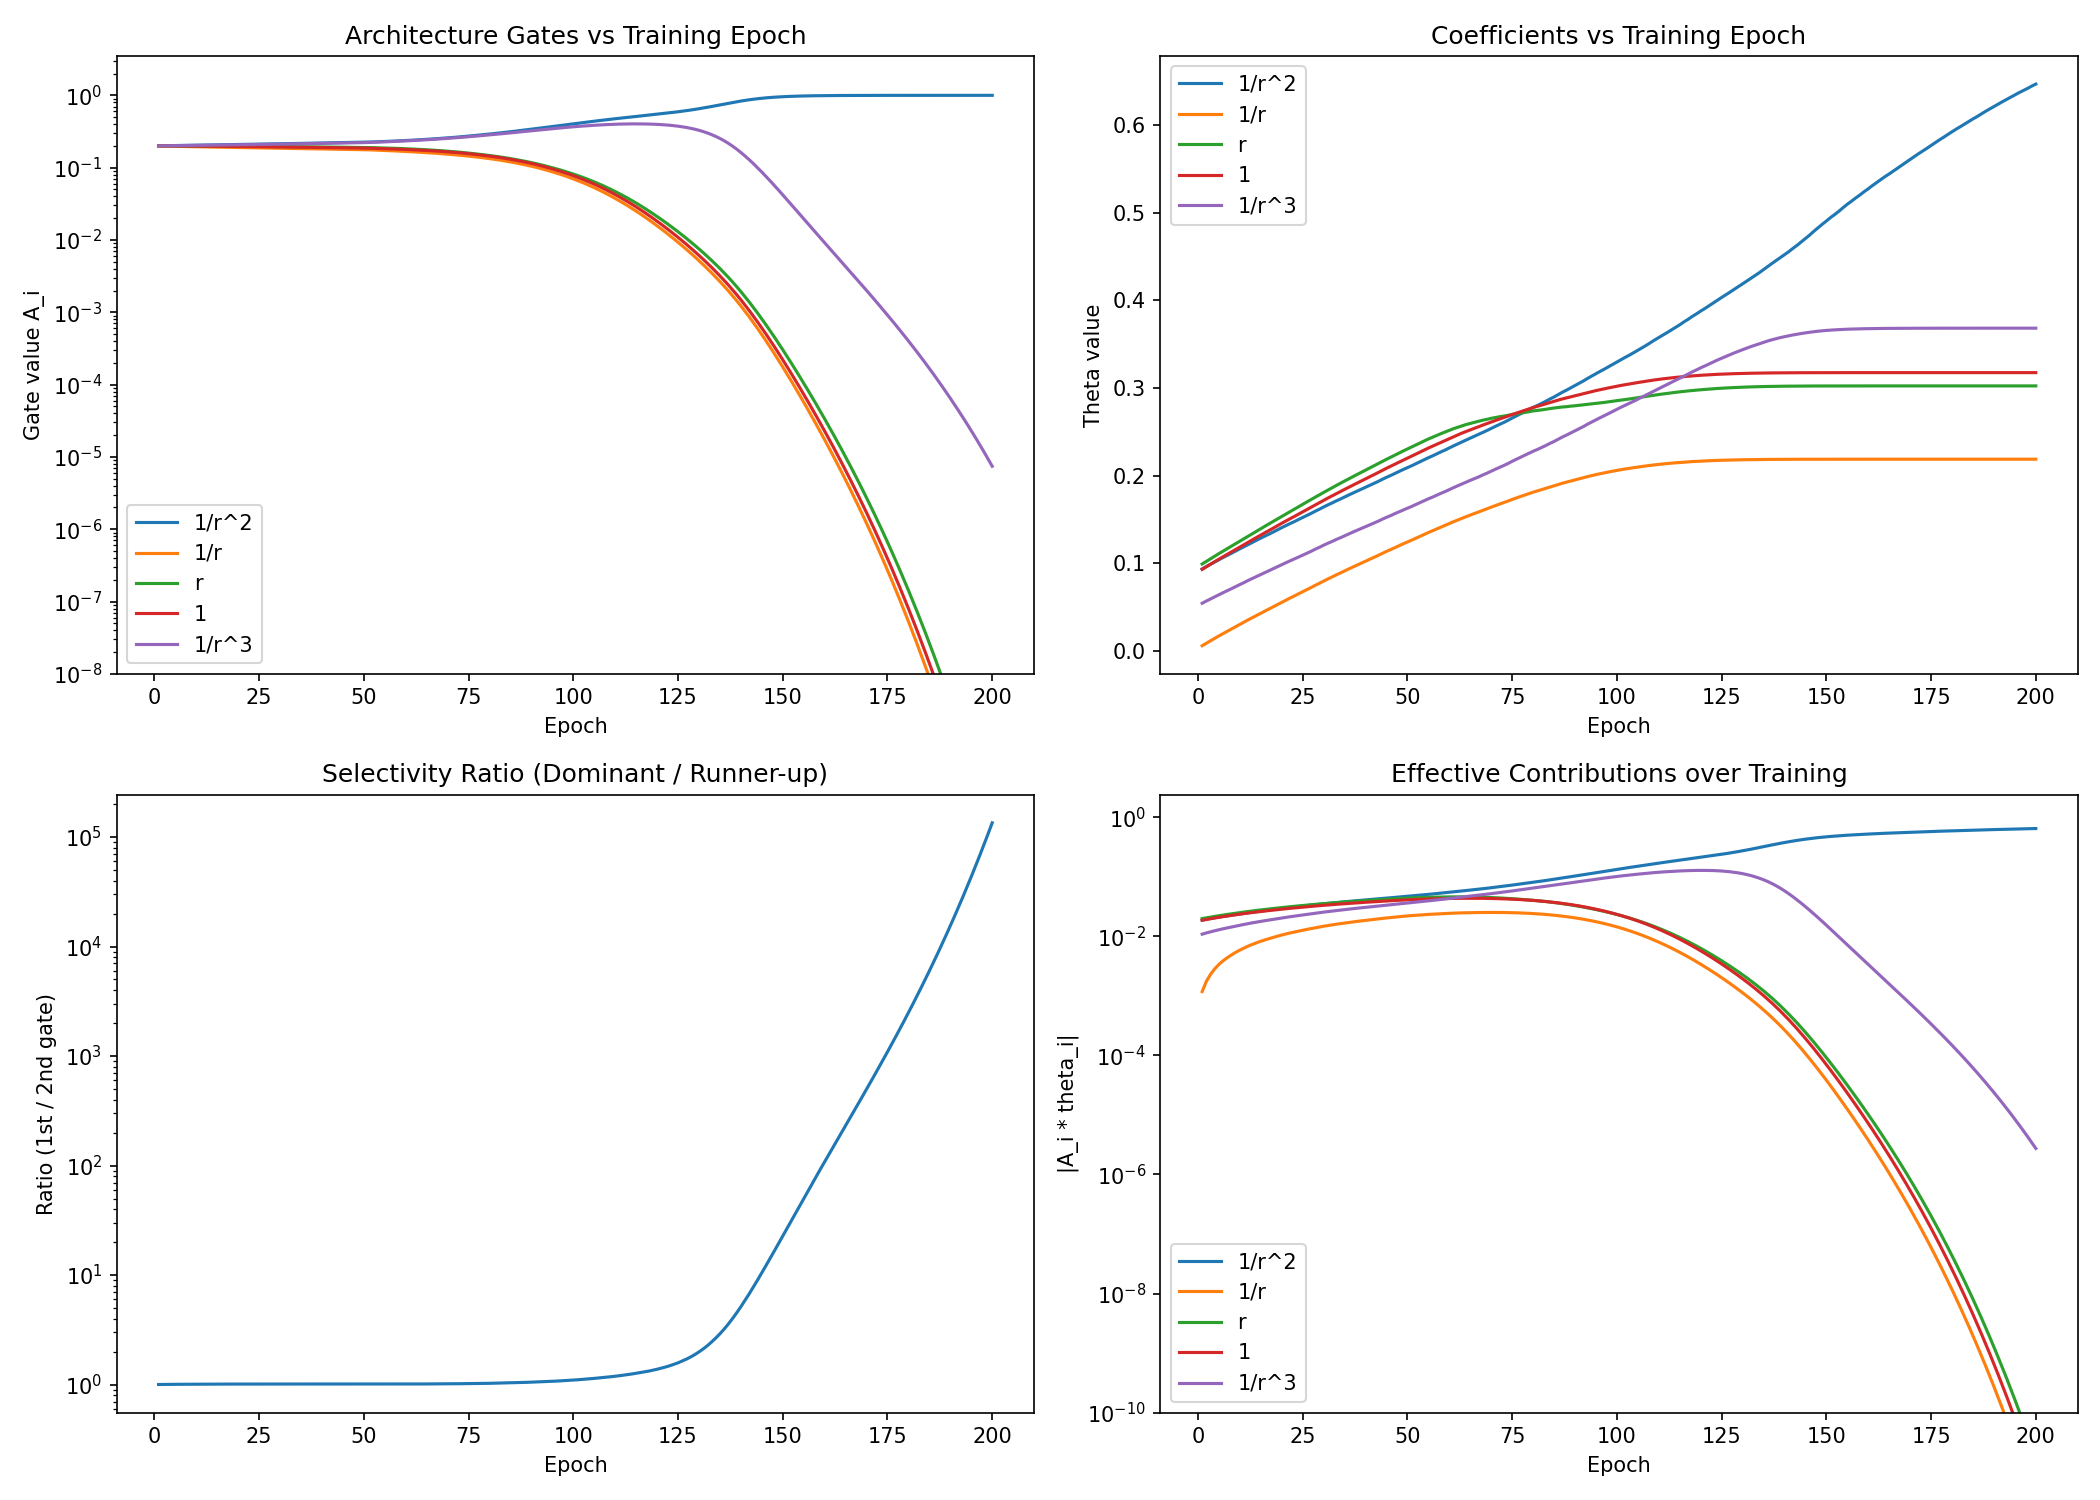
\includegraphics[width=0.9\linewidth]{figures/figS3_gates_seed137.png}
\caption{\textbf{Robustness: Seed 137 gate evolution.} Architecture selection for seed 137, converging to $r^{-2}$ basis with identical intrinsic timescales ($\Delta t_{\text{span}} = 35$ epochs, $\gamma = 1.141$).}
\label{fig:S3}
\end{figure}

\begin{figure}[!ht]
\centering
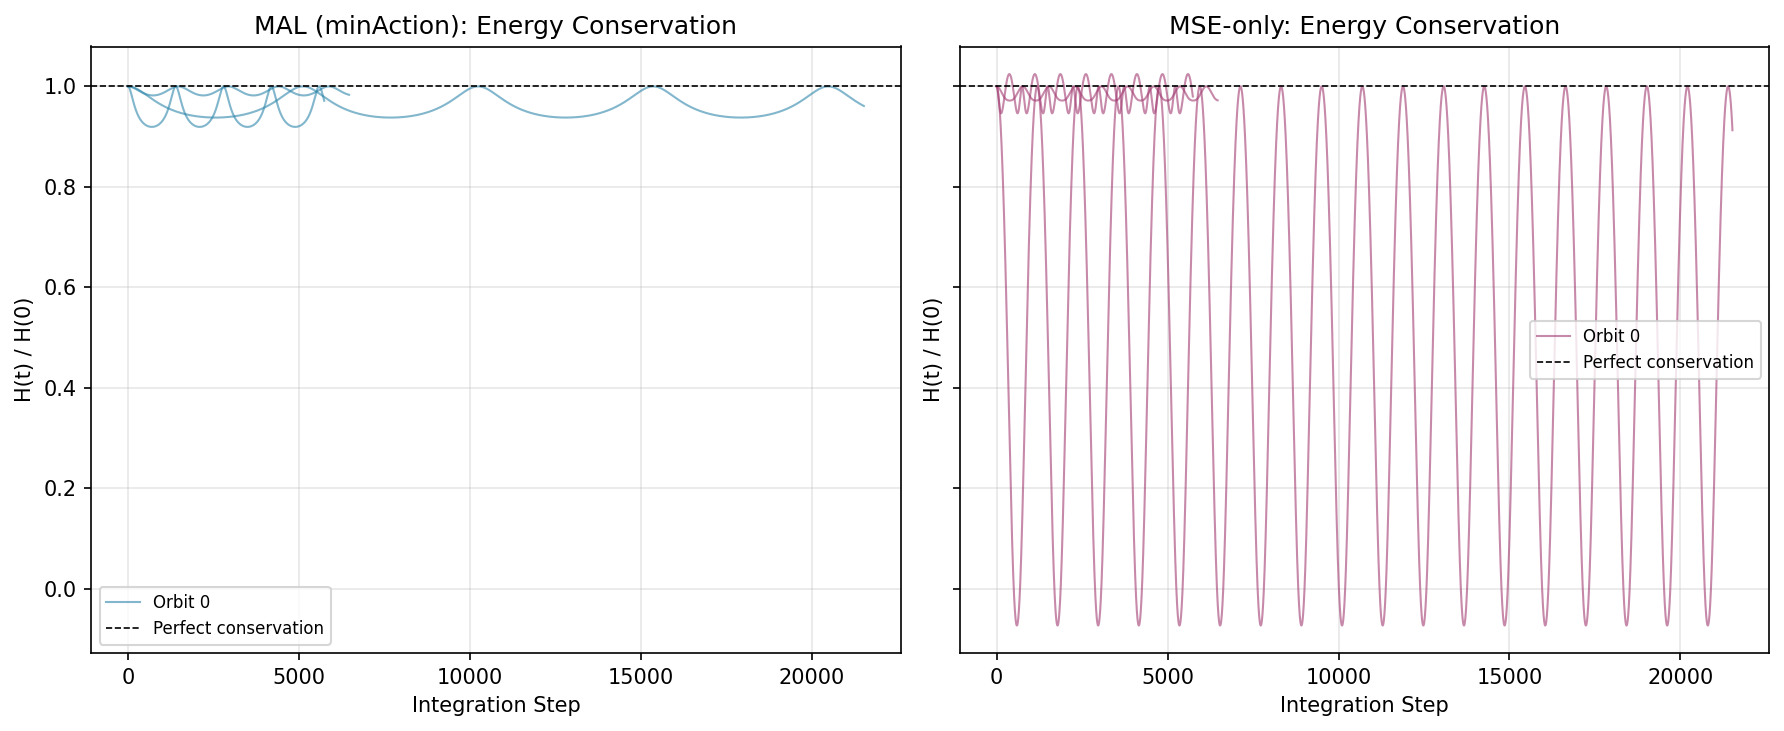
\includegraphics[width=0.9\linewidth]{figures/figS4_energy_seed137.png}
\caption{\textbf{Robustness: Seed 137 energy conservation.} Hamiltonian variance $\sigma_H = 0.019$ for seed 137, within the $r^{-2}$ group mean $0.017 \pm 0.016$, confirming energy-conservation selection criterion.}
\label{fig:S4}
\end{figure}

\begin{figure}[!ht]
\centering
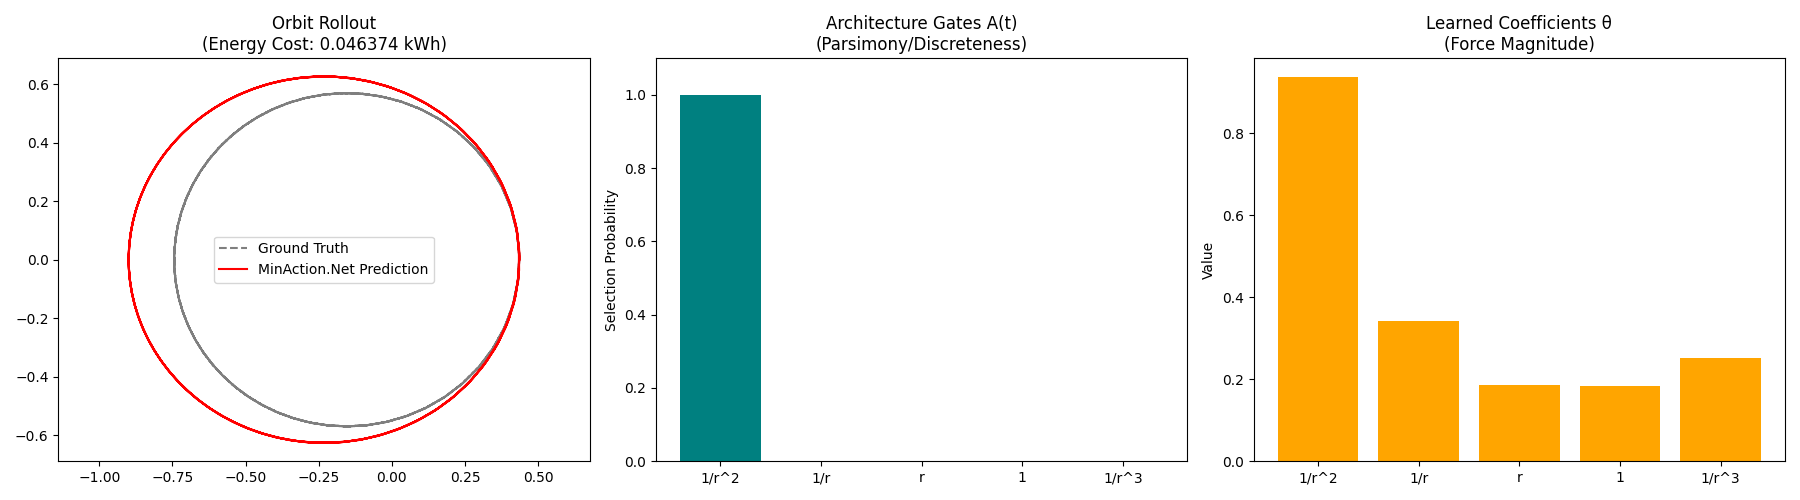
\includegraphics[width=0.9\linewidth]{figures/fig5_discovery_summary.png}
\caption{\textbf{Multi-panel discovery summary.} (A) Orbit comparison: model rollout vs.\ ground truth for test orbit. (B) Architecture gate evolution over 200 epochs. (C) Learned force coefficients $\theta_i$ before and after calibration. (D) Kepler exponent fit: $T^2 \propto a^{3.01}$.}
\label{fig:S5-summary}
\end{figure}

\begin{figure}[!ht]
\centering
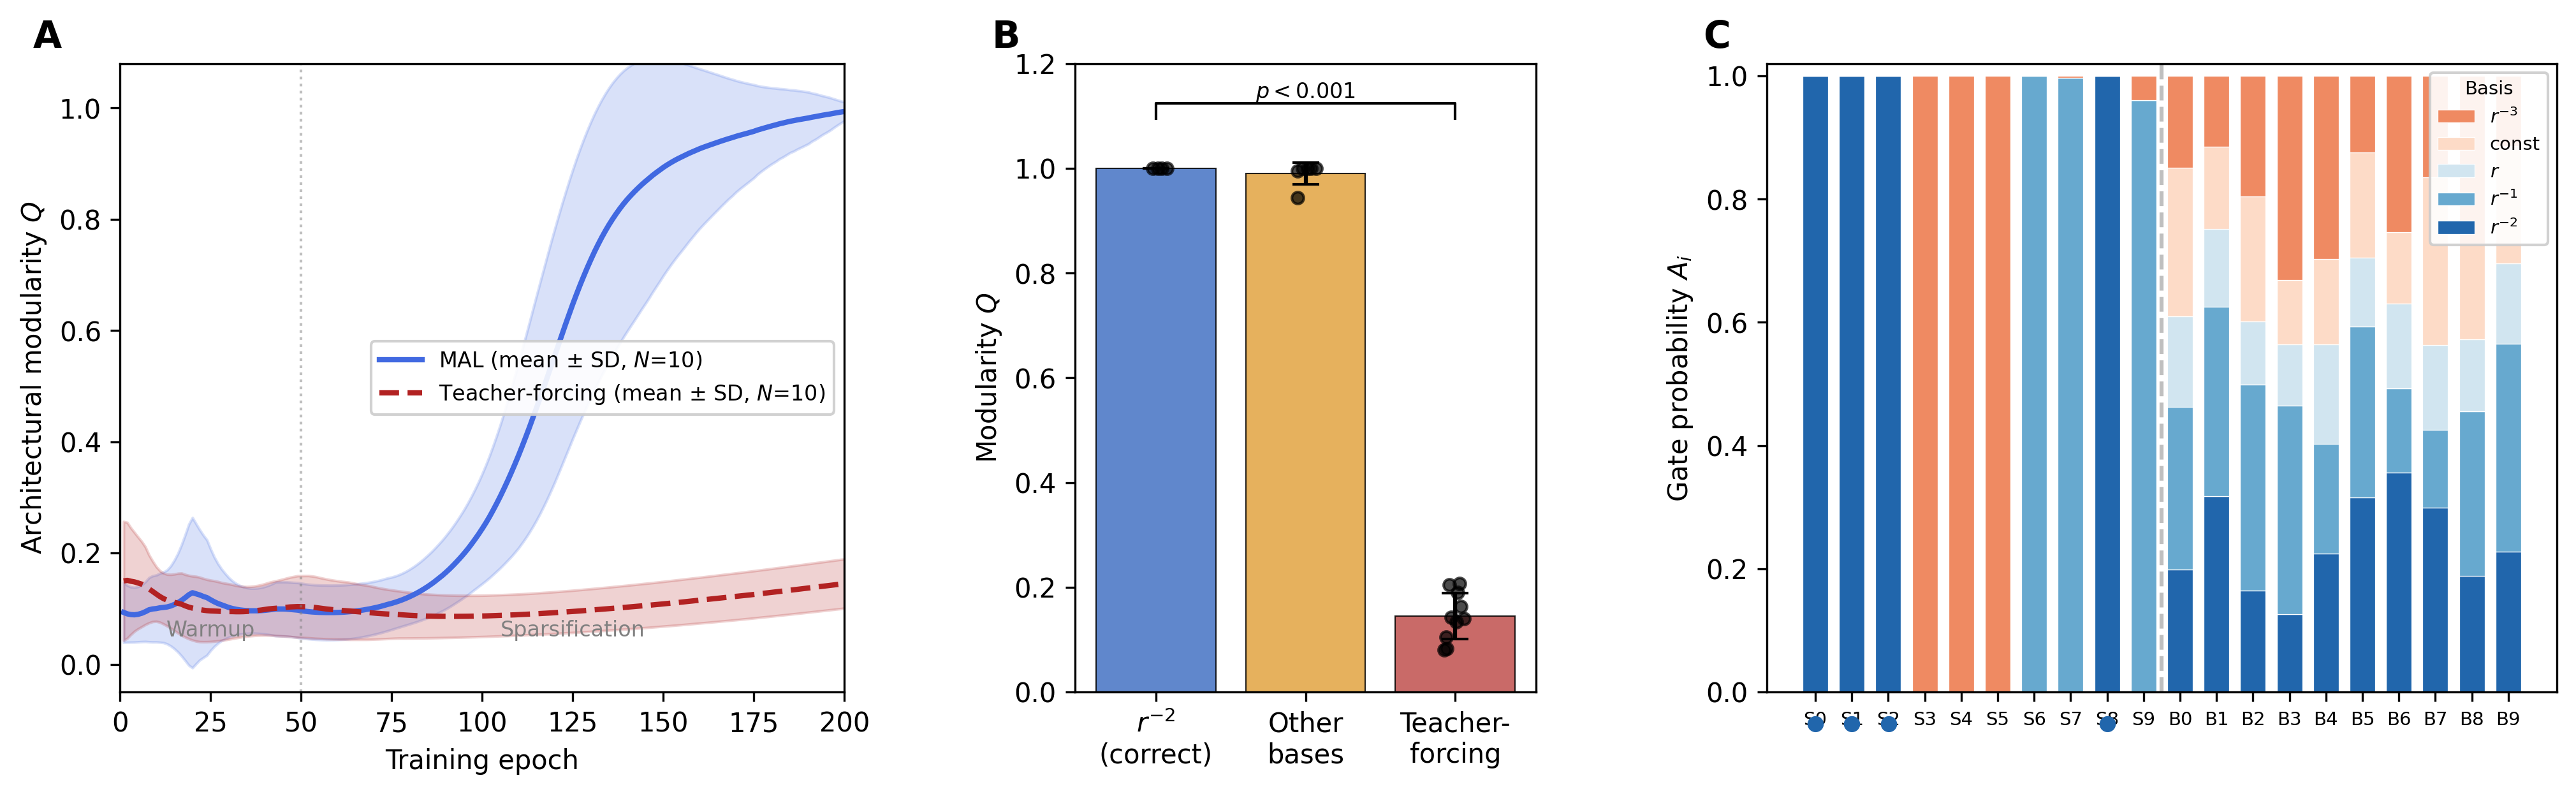
\includegraphics[width=0.9\linewidth]{figures/figS6_modularity.png}
\caption{\textbf{Architectural modularity analysis.} (A) Modularity index $Q$ (Herfindahl--Hirschman concentration on effective gate contributions $A_i|\theta_i|$) over training epochs for MAL (blue, mean $\pm$ SD, $N=10$ seeds) vs.\ teacher-forcing-only baselines (red dashed, $N=10$). Vertical dashed lines mark the warmup-to-sparsification transition. MAL modularity rises sharply during sparsification, reaching $Q = 0.99 \pm 0.02$ by epoch 200, while teacher-forcing remains diffuse ($Q = 0.14 \pm 0.04$). (B) Final modularity by group: models selecting the correct $r^{-2}$ basis, models selecting other bases, and teacher-forcing baselines (permutation test $p < 0.001$, $n = 10{,}000$). Both MAL groups achieve near-maximal $Q$ regardless of which basis is selected, confirming that energy-constrained training drives architectural sparsification independent of outcome. (C) Final gate probability distributions $A_i$ for all 10 MAL seeds (S0--S9) and 10 teacher-forcing baselines (B0--B9). MAL seeds crystallize to one-hot gate vectors (single dominant basis per seed), while baselines maintain diffuse distributions across all five bases.}
\label{fig:S6-modularity}
\end{figure}

\bibliography{references}

\end{document}
